
% The \phantomsection command is needed to create a link to a place in the document that is not a
% figure, equation, table, section, subsection, chapter, etc.
% https://tex.stackexchange.com/questions/44088/when-do-i-need-to-invoke-phantomsection
\phantomsection

\chapter{Integer Programming}\label{chap:integer-programming}


Integer Programming (IP), a subset of mathematical programming, addresses optimization problems where decision variables are required to take on integer values.
Specifically, mixed-integer linear programming (MILP) extends this concept by encompassing the assumption that for each possible discrete decision, a (continuous) linear program has to be solved.
The complexity of MILP problems often necessitates sophisticated solution methods to find optimal or near-optimal solutions.
This chapter provides an overview of MILP problem-solving techniques, ranging from exact methods like the branch-and-bound algorithm to approaches to provide approximate solutions, such as heuristics and matheuristics.
Through these methodologies, the groundwork is laid for the subsequent discussion on deep learning-based primal heuristics, which aim to enhance the efficiency of MILP problem solving.

\section{Integer and Combinatorial Optimization}

A solution for an integer and combinatorial optimization problem is the maximum or minimum value of a multivariate function that respects a series of inequality and equality constraints and integrality restrictions on some or all variables~\cite{nemhauserIntegerCombinatorialOptimization1999}.
It is not difficult to see that integer and combinatorial optimization encompasses a wide range of problems of practical utility.
Examples include train scheduling, airline crew scheduling, production planning, electricity generation planning, and cutting problems~\cite{wolseyIntegerProgramming1998}.

Mathematical programming is a language naturally suitable to formulate integer and combinatorial optimization problems, for example, in the form
\begin{equation}\label{eq:general-ip}
    \begin{split}
	\min_{\bm{x}} \quad & f\left( \bm{x} \right) \\
	\textrm{s.t.} \quad & \bm{g}\left( \bm{x} \right) \le \bm{0} \\
	  & \bm{x} \in \Z^{n}\times \R^{p}
    ,\end{split}
\end{equation}
with $n$ integer variables and $p$ continuous variables.
Furthermore, $\bm{g}: \Z^{n}\times \R^{p} \longrightarrow \R^{m}$,  and $\bm{0}$ is a null vector of dimension $m$.
Note that maximizing a function is equivalent to minimizing its negative, and an equality constraint can be represented by two inequalities, which renders \eqref{eq:general-ip} a complete formulation.

For an integer program formulated as in \eqref{eq:general-ip}, the set \[
\mathcal{X}=\left\{ \bm{x}\in \Z^{n}\times \R^{p}: \bm{g}\left( \bm{x} \right) \le \bm{0}\right\} 
\] is named the \emph{feasible region} of the problem, and a vector $\bm{x}\in \mathcal{X}$ is a \emph{feasible solution}.
A feasible solution $\bm{x}^{*}\in \mathcal{X}$ is \emph{optimal} if, and only if, there is no other feasible solution results in a lower value of the \emph{objective function} $f: \Z^{n}\times \R^{p} \longrightarrow \R$, i.e., $\bm{x}^{*}$ is optimal $\iff f(\bm{x}^{*}) \le f(\bm{x}) ,\,\forall \bm{x}\in \mathcal{X}$.

Note that even if a problem is feasible ($\mathcal{X}\neq \varnothing$), it may not have an optimal solution, e.g., if the feasible region is unbounded and the objective function has no global minimum.
Furthermore, if an optimal solution exists, it may no be unique.
% TODO: show how a problem may have no optimal solution even if with bounded feasible region. see Nemhauser, I.4.6

% TODO: show NP-hardness of IP by reducing SAT to it and citing "Computers and intractability: A guide to the theory of NP-completeness"

\section{Mixed-Integer Linear Programs}

MILP is a subset of IP in which the objective and the constraints are all linear functions and the problem requires integer and continuous variables.
Formally, an MILP can be formulated as 
\begin{equation}\label{eq:general-milp}
\begin{split}
    \min_{\bm{x}} \quad & \bm{c}^{T}\bm{x} \\
    \textrm{s.t.} \quad & A\bm{x} \le \bm{b} \\
	  & \bm{x} \in \Z^{n}\times \R^{p}
,\end{split}
\end{equation}
where $A\in \R^{m\times (n+p)}$ is the constraint matrix, $\bm{b}\in \R^{m}$ is the right-hand side vector, $\bm{c}\in \R^{n+p}$ is the cost vector, and $n>0$, $p>0$.
An \emph{instance} of an MILP problem is specified by a tuple  $\left( \bm{c},\bm{b},A,n \right)$.

As an example, take the MILP problem
\begin{equation}\label{eq:example-milp}
\begin{split}
    \min_{z,y} \quad & -y \\
    \textrm{s.t.} \quad & z - y\le 0 \\
      & z+y \le 5 \\
      & z \in \Z, y\ge 1
,\end{split}
\end{equation}
in which, to follow the notation of \eqref{eq:general-milp}, we have $\bm{x}=(z,y)$, \[
A=\begin{bmatrix} 1 & -1 \\ 1 & 1 \\0 & -1 \end{bmatrix}, \bm{b} = (0, 5, 0), \bm{c} = (0, -1) 
.\]
The feasible region of this problem is illustrated in Fig.~\ref{fig:milp-example}.

\begin{figure}[h]
    \centering
    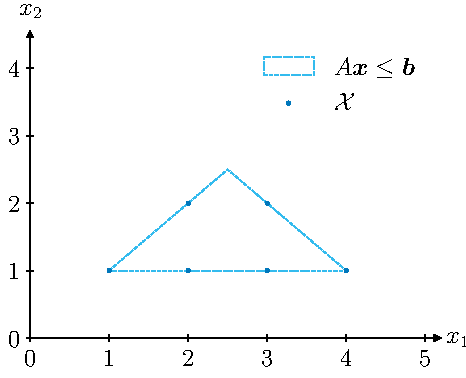
\includegraphics{pictures/milp_example_feasible_region.pdf}
    \caption{Feasible region of \eqref{eq:example-milp}.}
    \label{fig:milp-example}
\end{figure}

The significance of this class of problems has already been recognized by \citeonline{dantzigSignificanceSolvingLinear1960}.
% TODO: expand on Dantizig, 1960; state that it is on top of being NP-hard, as the SAT reduction renders a linear IP, and, thus, an MILP
% TODO: review the following statements
Naturally, MILP is necessary whenever linear programming (LP) problems require solutions to assume integer values.
On top of that, integer variables can be used to represent discrete choices over LP problems.
Finally, continuous nonlinear functions can be approximated to arbitrary quality by piecewise linear functions, and such functions 


\section{Solving MILP Problems}

\subsection{The Branch-and-Bound Algorithm}

\subsection{Heuristics}

\subsection{Matheuristics}

